\documentclass[12pt]{article}
%--------------------   start of the 'preamble'
%
\usepackage{graphicx,amssymb,amstext,amsmath,color}
\usepackage[margin=2cm]{geometry}
\usepackage{abstract}
\usepackage{setspace}
\usepackage[footnotesize,bf]{caption}

% TABLE
\usepackage{multicol,hhline,colortbl,multirow}
\usepackage{braket}
\usepackage{siunitx}
\usepackage{hyperref}
\usepackage{authblk}
\usepackage{siunitx}
\usepackage{mathrsfs}
%%\usepackage[sort&compress]{natbib}
%%\bibpunct{(}{)}{,}{a}{, }{;}
%
\usepackage[sort&compress]{natbib}
\bibpunct{[}{]}{,}{s}{}{;}


\definecolor{gray}{gray}{0.8}
\def\mobunits{\square\centi\meter\per\volt\per\second}
\def\gcm{\gram\per\cubic\centi\meter}
\def\ccg{\cellcolor{gray}}

\renewcommand{\labelitemii}{$\circ$}
\renewcommand{\bibname}{References}


\title{MorphCT - 1K P3HT 15mers}
\author{Matthew Jones}
\date{\today}

\begin{document}
\maketitle


\section{Simulations}


The simulations for the system containing 1,000 15mers of P3HT has compleded.
The system was UA to begin with, and so no fine-graining was required for this morphology.


\section{Mobility Results}


\begin{center}
\begin{tabular}{| c | c | c | c | c | c | c |}
\hline
\rule{0pt}{2.5ex} 
\multirow{2}{*}{\textbf{ID}}&\multirow{2}{*}{\textbf{Simulation Name}}&\textbf{Density}&\textbf{Anisotropy}&\textbf{Anisotropy}&\textbf{Stacks}&\textbf{Mobility}\\
                            &&(\SI{}{\gcm})&(Arb. U.)&(Shape)&(Arb. U.)&(\SI{}{\mobunits})\\
\hhline{|=======|}
\textbf{\ccg1}&\rule{0pt}{2.5ex}\ccg 1k\_P3HT&\ccg 1.11&\ccg 0.1086&\ccg Flat Disk&\ccg26&\ccg3.00$\times 10^{0}$\\
\hhline{-------}
\end{tabular}\label{table:mob}
\captionof{table}{The results from MorphCT.}
\end{center}

\clearpage


\begin{figure}[h]\centering
	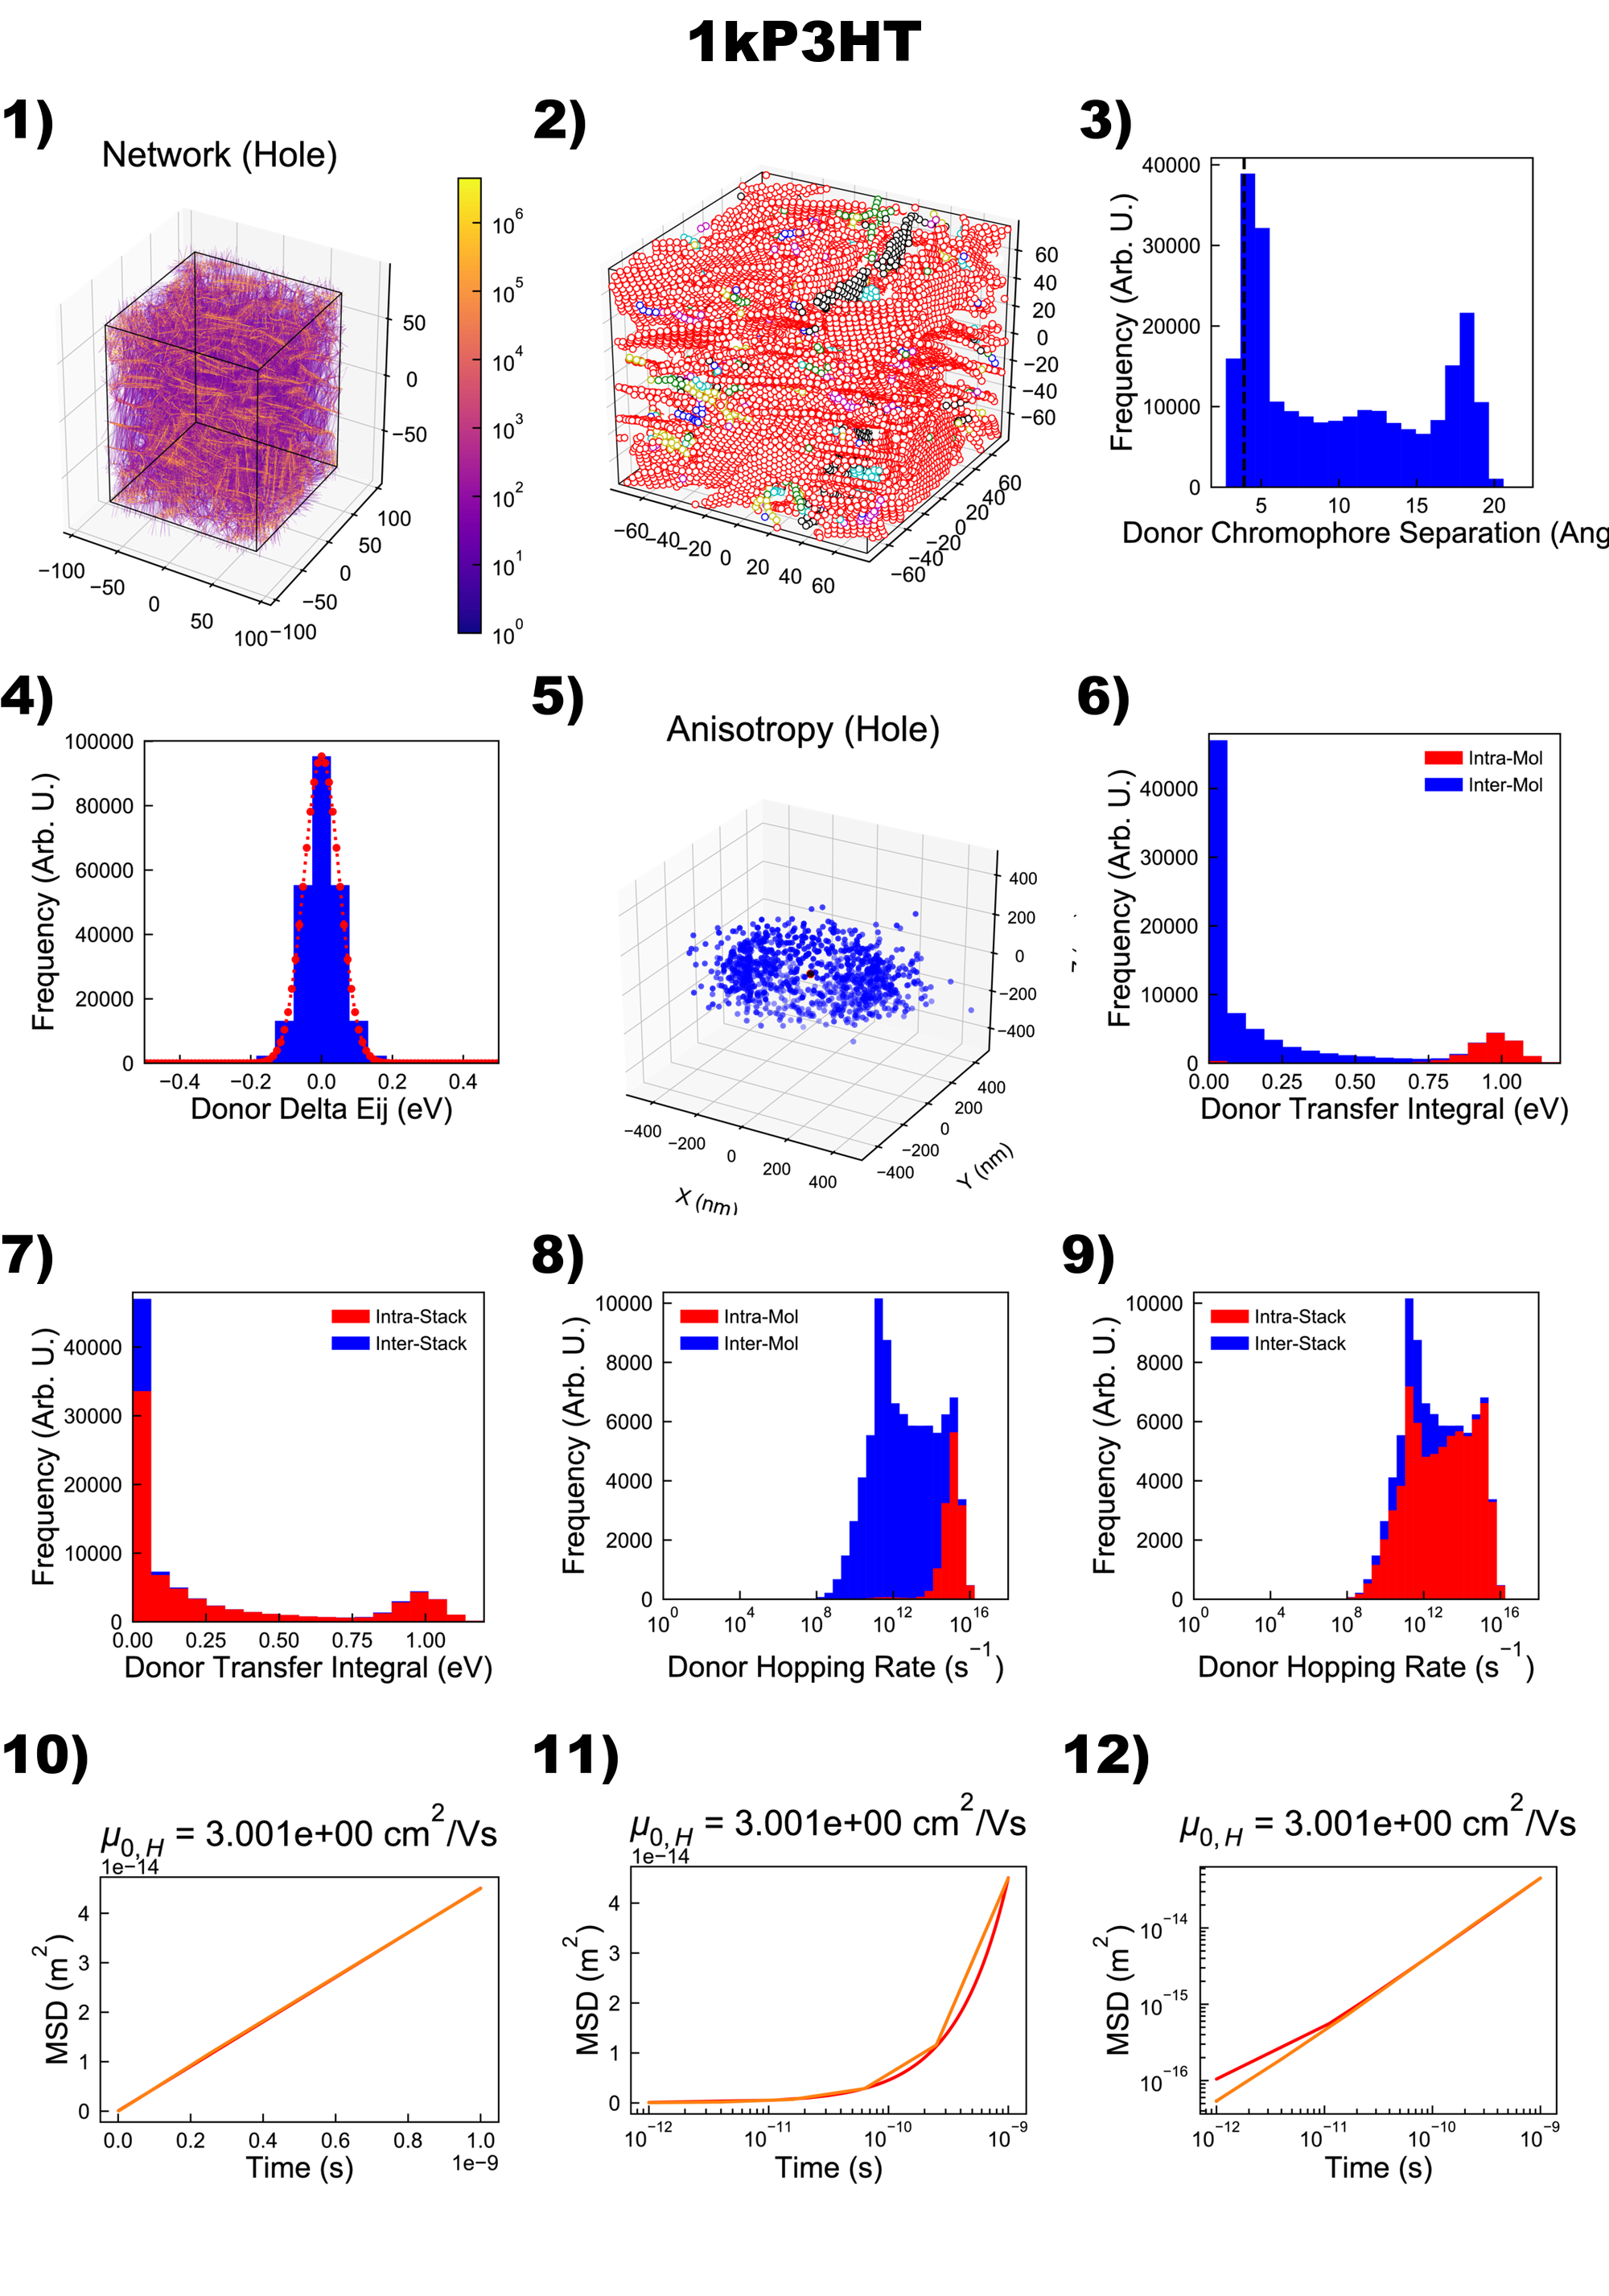
\includegraphics[width=0.85\textwidth]{Figures/1kP3HT.png}
    \caption{   1) Chromophore connectivity network, 
                2) Location of `stacks', 
                3) Distribution of connected chromophore separations (defines stacks),
                4) Density of states of Frontier molecular orbital (delta Eij),
                5) KMC Carrier termination locations (defines anisotropy),
                6) Histogram of molecular transfer integrals,
                7) Histogram of stack transfer integrals,
                8) Histogram of molecular hopping rates,
                9) Histogram of stack hopping rates,
                10) Linear MSD plot,
                11) Semi-log-x MSD plot,
                12) Logarithmic MSD plot.}
	\label{fig:1kP3HT}
\end{figure}

\bibliography{refs}
\bibliographystyle{unsrt}


\end{document}
